\documentclass[12pt,fleqn]{article}\usepackage{../../common}
\begin{document}
Sonlu Hacim (Finite Volume) Yöntemi - 3

Euler gaz denkleminin Riemann Roe yontemi ile cozumu

\begin{minted}[fontsize=\footnotesize]{python}
from collections import namedtuple
import matplotlib.pyplot as plt
import numpy as np

primitive_variables = ('Density', 'Velocity', 'Pressure')
Primitive_State = namedtuple('State', primitive_variables)

def primitive_to_conservative(rho, u, p, gamma=1.4):
    mom = rho*u
    E   = p/(gamma-1.) + 0.5*rho*u**2
    return rho, mom, E

def pospart(x):
    return np.maximum(1.e-15,x)

def conservative_to_primitive(rho, mom, E, gamma=1.4):
    u = mom/pospart(rho)
    p = (gamma-1.)*(E - 0.5*rho*u**2)
    return rho, u, p

def roe_averages(q_l, q_r, gamma=1.4):
    rho_sqrt_l = np.sqrt(q_l[0])
    rho_sqrt_r = np.sqrt(q_r[0])
    p_l = (gamma-1.)*(q_l[2]-0.5*(q_l[1]**2)/q_l[0])
    p_r = (gamma-1.)*(q_r[2]-0.5*(q_r[1]**2)/q_r[0])
    denom = rho_sqrt_l + rho_sqrt_r
    u_hat = (q_l[1]/rho_sqrt_l + q_r[1]/rho_sqrt_r)/denom
    H_hat = ((q_l[2]+p_l)/rho_sqrt_l + (q_r[2]+p_r)/rho_sqrt_r)/denom
    c_hat = np.sqrt((gamma-1)*(H_hat-0.5*u_hat**2))
    
    return u_hat, c_hat, H_hat
    
    
def Euler_roe(q_l, q_r, t, gamma=1.4):
    rho_l = q_l[0]
    rhou_l = q_l[1]
    u_l = rhou_l/rho_l
    rho_r = q_r[0]
    rhou_r = q_r[1]
    u_r = rhou_r/rho_r
    
    u_hat, c_hat, H_hat = roe_averages(q_l, q_r, gamma)

    dq = q_r - q_l
    
    s1 = u_hat - c_hat
    s2 = u_hat
    s3 = u_hat + c_hat
    
    alpha2 = (gamma-1.)/c_hat**2 *((H_hat-u_hat**2)*dq[0]+u_hat*dq[1]-dq[2])
    alpha3 = (dq[1] + (c_hat - u_hat)*dq[0] - c_hat*alpha2) / (2.*c_hat)
    alpha1 = dq[0] - alpha2 - alpha3
    
    r1 = np.array([1., u_hat-c_hat, H_hat - u_hat*c_hat])
    r2 = np.array([1., u_hat, 0.5*u_hat**2])
    q_l_star = q_l + alpha1*r1
    q_r_star = q_l_star + alpha2*r2
    
    states = np.column_stack([q_l,q_l_star,q_r_star,q_r])
    speeds = [s1, s2, s3]
    wave_types = ['contact','contact', 'contact']
    
    xmax = 0.9
    x = np.linspace(-xmax, xmax, 100)
    xi = x/(t+1e-10)
    rho = (xi<s1)*states[0,0] + (s1<=xi)*(xi<s2)*states[0,1] + \
          (s2<=xi)*(xi<s3)*states[0,2] + (s3<=xi)*states[0,3]
    mom = (xi<s1)*states[1,0] + (s1<=xi)*(xi<s2)*states[1,1] + \
          (s2<=xi)*(xi<s3)*states[1,2] + (s3<=xi)*states[1,3]
    E = (xi<s1)*states[2,0] + (s1<=xi)*(xi<s2)*states[2,1] + \
        (s2<=xi)*(xi<s3)*states[2,2] + (s3<=xi)*states[2,3]
    
    q = conservative_to_primitive(rho, mom, E, gamma=1.4)

    fig, axes = plt.subplots(3, 1, figsize=(5, 6), sharex=True)
    axes[0].plot(x,q[0]); axes[0].set_ylim(0,4); axes[0].set_title('t = ' + str(t))
    axes[1].plot(x,q[1]); axes[0].set_ylim(0,1)
    axes[2].plot(x,q[2]); axes[0].set_ylim(0,4)
    plt.savefig('euler-roe-%d.png' % (t*100))    
\end{minted}

\begin{minted}[fontsize=\footnotesize]{python}    
left  = Primitive_State(Density = 3.,
                        Velocity = 0.,
                        Pressure = 3.)

right = Primitive_State(Density = 1.,
                        Velocity = 0.,
                        Pressure = 1.)

q_l = np.array(primitive_to_conservative(*left))
q_r = np.array(primitive_to_conservative(*right))

Euler_roe(q_l, q_r, t=0.2)
Euler_roe(q_l, q_r, t=0.4)
Euler_roe(q_l, q_r, t=0.6)
Euler_roe(q_l, q_r, t=0.8)
\end{minted}

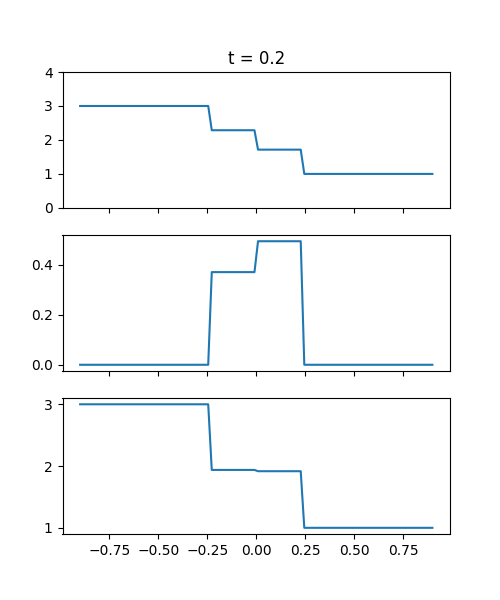
\includegraphics[width=20em]{euler-roe-20.png}

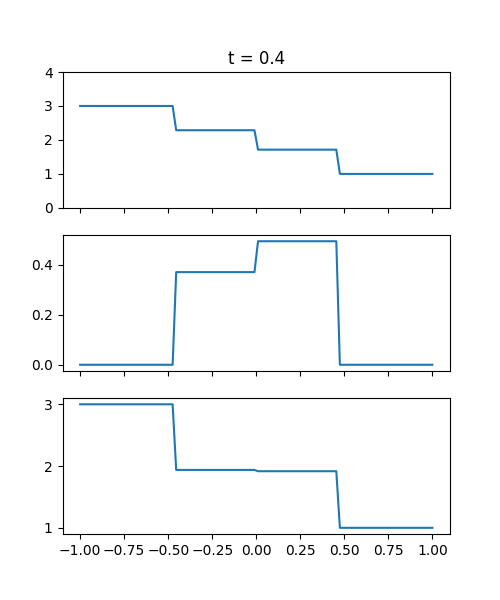
\includegraphics[width=20em]{euler-roe-40.png}

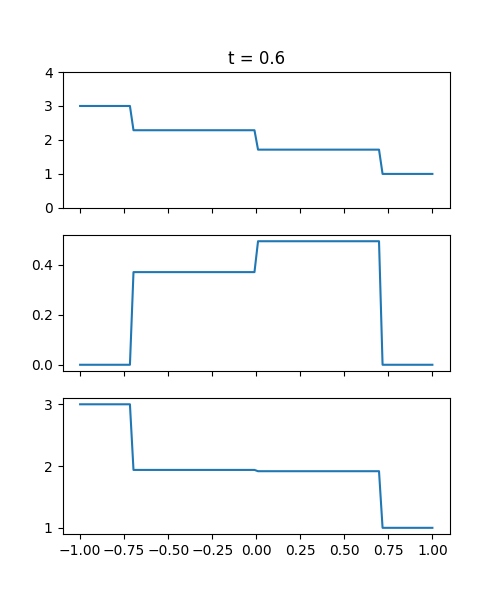
\includegraphics[width=20em]{euler-roe-60.png}

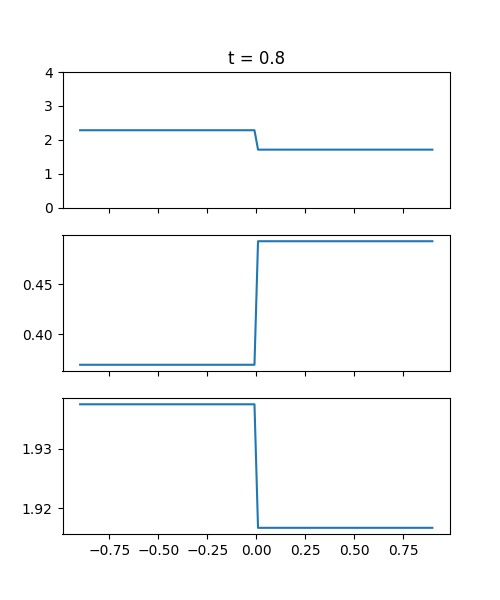
\includegraphics[width=20em]{euler-roe-80.png}












[devam edecek]


Kaynaklar

[1] Leveque, {\em Riemann Problems and Jupyter Solutions}


\end{document}
